%%%%%%%%%%%%%%%%%%%%%%%%
%
%   Thesis template by Youssif Al-Nashif
%
%   May 2020
%
%%%%%%%%%%%%%%%%%%%%%%%%

\chapter{Introduction}
\label{introduction}


% Big Ideas.
\hspace*{0.3cm} Text mining is the process of extracting insight from text documents using computational and statistical methods. A common task in text mining is document clustering, where the natural language of the documents is reformatted and used to group documents into clusters of similar topics or text content. These type of tasks are known as unsupervised clustering. Unsupervised clustering is the use of algorithms to take unlabeled data and estimate potential clusters, or groupings, of the observations of concern; supervised learning methods, like support vector machines or logistic regression, use labeled data to ``learn" how to discern between groups of data. Since the data are guiding the definition of clusters, or categories, this is an unsupervised approach. Popular methods to cluster text include k-means, hierarchical methods, and topic models. Most of these methods utilize term frequency-inverse document frequency measures  or bag-of-words methods to do clustering, though these methods often divide words and thus may lose meaning, or context, surrounding the word of concern. In an effort to cluster documents while still preserving the relationship between words, text can be modeled with graphs which better preserve the context surrounding a word. Text can be represented with bigram graphs, where the edge between two vertices is the result of two words appearing adjacent in the text. This idea can be extended to more general n-grams, and further extended to skip-n-grams, resulting in even richer representations of the text. The similarity of two of graphical representations can then be assessed using modern methods called graph kernels. Graph kernels produce a measure of similarity between graphs, thus allowing for further machine learning to take place. With a measure of similarity between two graphs, we can do an assortment of clustering methods.\\

The chosen graph representation of the observational unit of text is an extension of bigram graphs. The use of skip-grams here is a way to connect ideas between words that would have normally attained meaning through the ``context" of the sentence. By connecting words that appear close to one another while not being immediately adjacent, we are creating ``skip-grams"-- an extension of the bigram where the window for which words are considered adjacent is widened. A graphic in Figure 1.1 demonstrates this.\\

\begin{figure}
 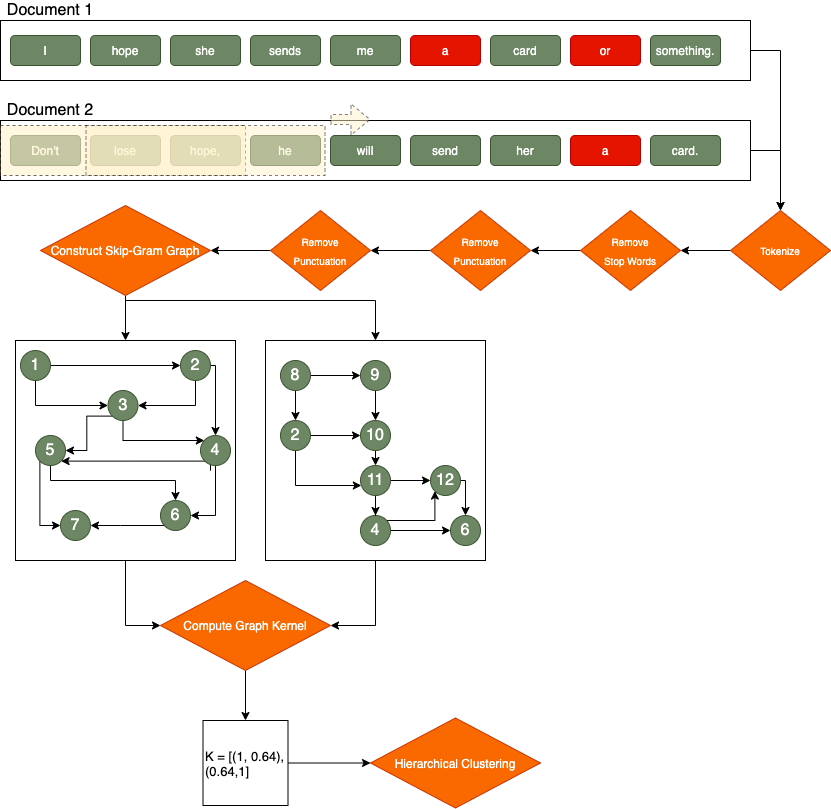
\includegraphics[width=6in]{Content/Images/Concept_map.png}
 \caption{A map of concepts used and how the methods used here work together. Example is a skip-gram graph of $k=2$.}
 \end{figure}

\hspace*{0.3cm} Many methods used in text mining use bag-of-words techniques, but these methods do not always preserve the context and relationships between words. The graph representations for text, used here, aim to preserve the relationship and context between words. The idea of bigrams (pairs of two words) can be extended to ``skip-grams”; skip-grams are words which appear within some width $w$ of each other. This leads to more connections, and a richer graph representation of the text. This skip-gram method is similar to that used in the popular machine learning package Word2Vec, which uses the “continuous bag of words” or ``continuous skip-grams”. In this paper, a graph representation of the text is constructed, using skip-gram methods, for each document in the datasets. \\

The graph representations are compared with a graph kernel, which is a measure of the similarity of two graphs. In this study, the graph kernel of choice is a ``edge histogram kernel”, because the kernel utilizes the labels of the vertices to assess the similarity of two graphs– not just the topology. Additionally, this is a computationally cheaper than other graph kernels. For each graph, the kernel produces a measure of similarity to the other $n-1$ graphs in the dataset. We can use machine learning methods which work nicely with kernels, e.g. support vector machine (supervised) or hierarchical clustering (unsupervised). The hierarchical clustering methods will be applied here for two datasets, and the results compared.\\

Alternatively, we could use this similarity measure between two graphs, to assess how similar other graphs in the dataset may be. That is, we can compare the similarity of graphs $B$ and $C$ through their similarity to $A$. To do this, a KDE (Kernel Density Estimation) to estimate a kernel density curve, the curve is then used to partition the rest of the dataset into clusters. The KDE bandwidth is modified to produce more or less local minima/maxima that can be then used to identify potential clusters. Basic calculus can be used to locate to inflection points that will serve as intervals for which a cluster will be defined. These methods were developed, but were not included in the final analysis; they are available in the appendices and in a GitHub repository. \\

To test these methods, two different text data sets will be considered. First, reddit comments from subreddits pertaining to mental health. Using the \texttt{\{redditExtractoR\}} package \cite{rivera2015package}, the comments are collected if they match criteria set by the query. From the subreddit \texttt{r/mentalhealth}, posts are collected if they have chosen keywords and at least 10 comments. The keywords considered are ``anxious", ``anxiety", ``depressed", ``depression", ``mental", ``illness", ``scared", ``afraid", ``sad", ``emotion", ``anger", ``angry", ``upset", ``suicide", ``abuse", ``emotional", ``help", and ``addiction". These words do not represent all words which define or indicate mental health topics may be present; these words were chosen by the researcher arbitrarily. The result of the queries is thousands of comments. Mental health continues to be a growing focus at the national level, and the discussion on reddit is often candid and open, due to reddit's reputation as an anonymous website. The second data set being considered in the study, is NHTSA report data. These reports are form the Special Crash Investigation (SCI) reports from the NHTSA (National Highway Traffic Safety Administration). The pdf documents that are considered in this study are those that involved ambulance(s) in the incidents highlighted in the reports. These events are considered ``edge cases" and could prove useful to those working in autonomous vehicles. \\

These datasets were chosen because they are two very different styles of writing. The reddit posts are often in contemporary and casual use of language, possibly including ``netspeak", while the NHTSA reports feature a technical writing style with plain language, absent of hyperbole or sarcasm. These datasets show two very different sides of text data, and comparisons will be made to how each dataset responds to the methods outlined above. \\

Throughout the analysis, all the code used and datasets were documented for future use. The code is well documented in the form of explanatory code notebooks (RMarkdown), code comments, and supplementary markdown files. Datasets, scripts, notebooks, and supplementary files are all made available through a public GitHub repository. Part of the primary focus while developing these methods was to produce them a manner which follows good practices for reproducibility and open source software development. The scripts can all be used in a manner that allows a workflow from raw text to clustered documents; the workflow is documented in the form of a ``script map" or a process flow diagram, so new users can understand the process more clearly. 